\documentclass[]{article}
\usepackage{lmodern}
\usepackage{amssymb,amsmath}
\usepackage{ifxetex,ifluatex}
\usepackage{fixltx2e} % provides \textsubscript
\ifnum 0\ifxetex 1\fi\ifluatex 1\fi=0 % if pdftex
  \usepackage[T1]{fontenc}
  \usepackage[utf8]{inputenc}
\else % if luatex or xelatex
  \ifxetex
    \usepackage{mathspec}
    \usepackage{xltxtra,xunicode}
  \else
    \usepackage{fontspec}
  \fi
  \defaultfontfeatures{Mapping=tex-text,Scale=MatchLowercase}
  \newcommand{\euro}{€}
\fi
% use upquote if available, for straight quotes in verbatim environments
\IfFileExists{upquote.sty}{\usepackage{upquote}}{}
% use microtype if available
\IfFileExists{microtype.sty}{\usepackage{microtype}}{}
\usepackage[margin=1in]{geometry}
\usepackage{color}
\usepackage{fancyvrb}
\newcommand{\VerbBar}{|}
\newcommand{\VERB}{\Verb[commandchars=\\\{\}]}
\DefineVerbatimEnvironment{Highlighting}{Verbatim}{commandchars=\\\{\}}
% Add ',fontsize=\small' for more characters per line
\newenvironment{Shaded}{}{}
\newcommand{\AlertTok}[1]{\textcolor[rgb]{1.00,0.00,0.00}{\textbf{#1}}}
\newcommand{\AnnotationTok}[1]{\textcolor[rgb]{0.38,0.63,0.69}{\textbf{\textit{#1}}}}
\newcommand{\AttributeTok}[1]{\textcolor[rgb]{0.49,0.56,0.16}{#1}}
\newcommand{\BaseNTok}[1]{\textcolor[rgb]{0.25,0.63,0.44}{#1}}
\newcommand{\BuiltInTok}[1]{#1}
\newcommand{\CharTok}[1]{\textcolor[rgb]{0.25,0.44,0.63}{#1}}
\newcommand{\CommentTok}[1]{\textcolor[rgb]{0.38,0.63,0.69}{\textit{#1}}}
\newcommand{\CommentVarTok}[1]{\textcolor[rgb]{0.38,0.63,0.69}{\textbf{\textit{#1}}}}
\newcommand{\ConstantTok}[1]{\textcolor[rgb]{0.53,0.00,0.00}{#1}}
\newcommand{\ControlFlowTok}[1]{\textcolor[rgb]{0.00,0.44,0.13}{\textbf{#1}}}
\newcommand{\DataTypeTok}[1]{\textcolor[rgb]{0.56,0.13,0.00}{#1}}
\newcommand{\DecValTok}[1]{\textcolor[rgb]{0.25,0.63,0.44}{#1}}
\newcommand{\DocumentationTok}[1]{\textcolor[rgb]{0.73,0.13,0.13}{\textit{#1}}}
\newcommand{\ErrorTok}[1]{\textcolor[rgb]{1.00,0.00,0.00}{\textbf{#1}}}
\newcommand{\ExtensionTok}[1]{#1}
\newcommand{\FloatTok}[1]{\textcolor[rgb]{0.25,0.63,0.44}{#1}}
\newcommand{\FunctionTok}[1]{\textcolor[rgb]{0.02,0.16,0.49}{#1}}
\newcommand{\ImportTok}[1]{#1}
\newcommand{\InformationTok}[1]{\textcolor[rgb]{0.38,0.63,0.69}{\textbf{\textit{#1}}}}
\newcommand{\KeywordTok}[1]{\textcolor[rgb]{0.00,0.44,0.13}{\textbf{#1}}}
\newcommand{\NormalTok}[1]{#1}
\newcommand{\OperatorTok}[1]{\textcolor[rgb]{0.40,0.40,0.40}{#1}}
\newcommand{\OtherTok}[1]{\textcolor[rgb]{0.00,0.44,0.13}{#1}}
\newcommand{\PreprocessorTok}[1]{\textcolor[rgb]{0.74,0.48,0.00}{#1}}
\newcommand{\RegionMarkerTok}[1]{#1}
\newcommand{\SpecialCharTok}[1]{\textcolor[rgb]{0.25,0.44,0.63}{#1}}
\newcommand{\SpecialStringTok}[1]{\textcolor[rgb]{0.73,0.40,0.53}{#1}}
\newcommand{\StringTok}[1]{\textcolor[rgb]{0.25,0.44,0.63}{#1}}
\newcommand{\VariableTok}[1]{\textcolor[rgb]{0.10,0.09,0.49}{#1}}
\newcommand{\VerbatimStringTok}[1]{\textcolor[rgb]{0.25,0.44,0.63}{#1}}
\newcommand{\WarningTok}[1]{\textcolor[rgb]{0.38,0.63,0.69}{\textbf{\textit{#1}}}}
\usepackage{graphicx}
\makeatletter
\def\maxwidth{\ifdim\Gin@nat@width>\linewidth\linewidth\else\Gin@nat@width\fi}
\def\maxheight{\ifdim\Gin@nat@height>\textheight\textheight\else\Gin@nat@height\fi}
\makeatother
% Scale images if necessary, so that they will not overflow the page
% margins by default, and it is still possible to overwrite the defaults
% using explicit options in \includegraphics[width, height, ...]{}
\setkeys{Gin}{width=\maxwidth,height=\maxheight,keepaspectratio}
\ifxetex
  \usepackage[setpagesize=false, % page size defined by xetex
              unicode=false, % unicode breaks when used with xetex
              xetex]{hyperref}
\else
  \usepackage[unicode=true]{hyperref}
\fi
\hypersetup{breaklinks=true,
            bookmarks=true,
            pdfauthor={Justin Le},
            pdftitle={Tries with Recursion Schemes},
            colorlinks=true,
            citecolor=blue,
            urlcolor=blue,
            linkcolor=magenta,
            pdfborder={0 0 0}}
\urlstyle{same}  % don't use monospace font for urls
% Make links footnotes instead of hotlinks:
\renewcommand{\href}[2]{#2\footnote{\url{#1}}}
\setlength{\parindent}{0pt}
\setlength{\parskip}{6pt plus 2pt minus 1pt}
\setlength{\emergencystretch}{3em}  % prevent overfull lines
\setcounter{secnumdepth}{0}

\title{Tries with Recursion Schemes}
\author{Justin Le}

\begin{document}
\maketitle

\emph{Originally posted on
\textbf{\href{https://blog.jle.im/entry/tries-with-recursion-schemes.html}{in
Code}}.}

Not too long ago, I was browsing the
\href{https://www.reddit.com/r/PrequelMemes}{prequel memes subreddit} --- a
community built around creative ways of remixing and re-contextualizing quotes
from the cinematic corpus of the three Star Wars prequel movies --- when I
noticed that a fad was in progress
\href{https://www.reddit.com/r/PrequelMemes/comments/9w59t4/i_expanded_it/}{constructing
tries based on quotes as keys} indexing stills from the movie corresponding to
those quotes.

This inspired me to try playing around with some tries myself, and it gave me an
excuse to play around with
\emph{\href{https://hackage.haskell.org/package/recursion-schemes}{recursion-schemes}}
(one of my favorite Haskell libraries). If you haven't heard about it yet,
\emph{recursion-schemes} (and the similar library
\emph{\href{https://hackage.haskell.org/package/data-fix}{data-fix}}) abstracts
over common recursive functions written on recursive data types. It exploits the
fact that a lot of recursive functions for different recursive data types all
really follow the same pattern and gives us powerful tools for writing cleaner
and safer code.

Recursion schemes is a perfect example of those amazing accidents that happen
throughout the Haskell ecosystem: an extremely ``theoretically beautiful''
abstraction that also happens to be extremely useful for writing industrially
rigorous code.

Tries are a common intermediate-level recursive data type, and recursion-schemes
is a common intermediate-level library. So, as a fun intermediate-level Haskell
project, let's build a trie data type in Haskell based on recursion-schemes, to
see what it has to offer! The resulting data type will definitely not be a
``toy'' --- it'll be something you can actually use to build meme diagrams of
your own!

\hypertarget{trie}{%
\section{Trie}\label{trie}}

A \href{https://en.wikipedia.org/wiki/Trie}{trie} (prefix tree) is a classic
example of a simple yet powerful data type most people encounter in school (I
remember being introduced to it through a project implementing a boggle solver).

Wikipedia has a nice picture:

\begin{figure}
\centering
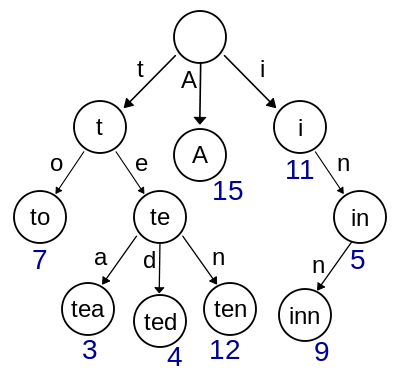
\includegraphics{/img/entries/trie/wiki-trie.png}
\caption{Sample Trie from Wikipedia, indexing lists of Char to Ints}
\end{figure}

API-wise, it is very similar to an \emph{associative map}, like the \texttt{Map}
type from
\emph{\href{https://hackage.haskell.org/package/containers/docs/Data-Map-Lazy.html}{containers}}.
It stores ``keys'' to ``values'', and you can insert a value at a given key,
lookup the value stored at a given key, or delete the value at a given key.

The main difference is in implementation: the keys are \emph{strings of tokens},
and it is internally represented as a tree: if your keys are words, then the
first level is the first letter, the second level is the letter, etc. In the
example above, the trie stores the keys \texttt{to}, \texttt{tea}, \texttt{ted},
\texttt{ten}, \texttt{A}, \texttt{i}, \texttt{in}, and \texttt{inn}, to the
values 7, 3, 4, 12, 15, 11, 5, and 9, respectively. Note that it is possible for
one key to completely overlap another (like \texttt{in} storing 5, and
\texttt{inn} storing 9). In the usual case, however, we have partial overlaps
(like \texttt{tea}, storing 3, and \texttt{ted} storing 4), whose common prefix
(\texttt{te}) has no value stored under it.

\hypertarget{haskell-tries}{%
\section{Haskell Tries}\label{haskell-tries}}

We can represent this in Haskell by representing each layer as a \texttt{Map} of
a token to the next ``level'' of the trie:

\begin{Shaded}
\begin{Highlighting}[]
\CommentTok{-- source: https://github.com/mstksg/inCode/tree/master/code-samples/trie/trie.hs#L32-L33}

\KeywordTok{data} \DataTypeTok{Trie}\NormalTok{ k v }\FunctionTok{=} \DataTypeTok{MkT}\NormalTok{ (}\DataTypeTok{Maybe}\NormalTok{ v) (}\DataTypeTok{Map}\NormalTok{ k (}\DataTypeTok{Trie}\NormalTok{ k v))}
  \KeywordTok{deriving} \DataTypeTok{Show}
\end{Highlighting}
\end{Shaded}

A \texttt{Trie\ k\ v} will have keys of type \texttt{{[}k{]}}, where \texttt{k}
is the key token type, and values of type \texttt{v}. Each layer might have a
value (\texttt{Maybe\ v}), and branches out to each new layer.

We could write the trie storing \texttt{(to,\ 9)}, \texttt{(ton,\ 3)}, and
\texttt{(tax,\ 2)} as:

\begin{Shaded}
\begin{Highlighting}[]
\CommentTok{-- source: https://github.com/mstksg/inCode/tree/master/code-samples/trie/trie.hs#L48-L62}

\OtherTok{testTrie ::} \DataTypeTok{Trie} \DataTypeTok{Char} \DataTypeTok{Int}
\NormalTok{testTrie }\FunctionTok{=} \DataTypeTok{MkT} \DataTypeTok{Nothing} \FunctionTok{$}\NormalTok{ M.fromList [}
\NormalTok{      (}\CharTok{'t'}\NormalTok{, }\DataTypeTok{MkT} \DataTypeTok{Nothing} \FunctionTok{$}\NormalTok{ M.fromList [}
\NormalTok{          (}\CharTok{'o'}\NormalTok{, }\DataTypeTok{MkT}\NormalTok{ (}\DataTypeTok{Just} \DecValTok{9}\NormalTok{) }\FunctionTok{$}\NormalTok{ M.fromList [}
\NormalTok{              ( }\CharTok{'n'}\NormalTok{, }\DataTypeTok{MkT}\NormalTok{ (}\DataTypeTok{Just} \DecValTok{3}\NormalTok{) M.empty )}

\NormalTok{            ]}
\NormalTok{          )}
\NormalTok{        , (}\CharTok{'a'}\NormalTok{, }\DataTypeTok{MkT} \DataTypeTok{Nothing} \FunctionTok{$}\NormalTok{ M.fromList [}
\NormalTok{              ( }\CharTok{'x'}\NormalTok{, }\DataTypeTok{MkT}\NormalTok{ (}\DataTypeTok{Just} \DecValTok{2}\NormalTok{) M.empty )}
\NormalTok{            ]}
\NormalTok{          )}
\NormalTok{        ]}
\NormalTok{      )}
\NormalTok{    ]}
\end{Highlighting}
\end{Shaded}

Note that this implementation isn't particularly structurally sound, since it's
possible to represent invalid keys that have branches that lead to nothing. This
mostly becomes troublesome when we implement \texttt{delete}, but we won't be
worrying about that for now. The nice thing about Haskell is that we can be as
safe as we want or need, as a judgement call on a case-by-case basis. However, a
``correct-by-construction'' trie is in the next part of this series :)

\hypertarget{enter-recursion-schemes}{%
\subsection{Enter Recursion Schemes}\label{enter-recursion-schemes}}

Now, \texttt{Trie} as we write it up there is an explicitly recursive data type.
While this is common practice, it's not a particularly ideal one. The problem
with explicitly recursive data types is that to work with them, you often rely
on explicitly recursive functions.

Explicitly recursive functions are notoriously difficult to write, understand,
and maintain. It's extremely easy to accidentally write an infinite loop, and is
often called ``the GOTO of functional programming''.

So, there's a trick we can use to ``factor out'' the recursion in our data type.
The trick is to replace the recursive occurrence of \texttt{Trie\ a} (in the
\texttt{Cons} constructor) with a ``placeholder'' variable:

\begin{Shaded}
\begin{Highlighting}[]
\CommentTok{-- source: https://github.com/mstksg/inCode/tree/master/code-samples/trie/trie.hs#L35-L36}

\KeywordTok{data} \DataTypeTok{TrieF}\NormalTok{ k v x }\FunctionTok{=} \DataTypeTok{MkTF}\NormalTok{ (}\DataTypeTok{Maybe}\NormalTok{ v) (}\DataTypeTok{Map}\NormalTok{ k x)}
  \KeywordTok{deriving}\NormalTok{ (}\DataTypeTok{Functor}\NormalTok{, }\DataTypeTok{Show}\NormalTok{)}
\end{Highlighting}
\end{Shaded}

\texttt{TrieF} now represents, essentially, ``one layer'' of a \texttt{Trie}.

There are now two paths we can go down: we can re-implement \texttt{Trie} in
terms of \texttt{TrieF} (something that most tutorials and introductions do), or
we can think of \texttt{TrieF} as a ``non-recursive view'' into \texttt{Trie}.
It's a way of \emph{working} with \texttt{Trie\ a} \emph{as if} it were a
non-recursive data type.

That's because \emph{recursion-schemes} gives combinators (called ``recursion
schemes'') to abstract over common explicit recursion patterns. The key to using
\emph{recursion-schemes} is to recognize which combinators abstracts over the
type of recursion you're using. You then give that combinator an algebra or a
coalgebra (more on this later), and you're done!

Learning how to use \emph{recursion-schemes} effectively is basically picking
the right recursion scheme that abstracts over the type of function you want to
write for your data type. It's all about becoming familiar with the ``zoo'' of
(colorfully named) recursion schemes you can pick from, and identifying which
one does the job in your situation.

That's the high-level view --- let's dive into writing out the API of our
\texttt{Trie}!

\hypertarget{linking-the-base}{%
\subsection{Linking the base}\label{linking-the-base}}

One thing we need to do before we can start: we need to tell
\emph{recursion-schemes} to link \texttt{TrieF} with \texttt{Trie}. In the
nomenclature of \emph{recursion-schemes}, \texttt{TrieF} is known as the ``base
type'', and \texttt{Trie} is called ``the fixed-point''.

Linking them requires some boilerplate, which is basically converting back and
forth from \texttt{Trie} to \texttt{TrieF}.

\begin{Shaded}
\begin{Highlighting}[]
\CommentTok{-- source: https://github.com/mstksg/inCode/tree/master/code-samples/trie/trie.hs#L38-L46}

\KeywordTok{type} \KeywordTok{instance} \DataTypeTok{Base}\NormalTok{ (}\DataTypeTok{Trie}\NormalTok{ k v) }\FunctionTok{=} \DataTypeTok{TrieF}\NormalTok{ k v}

\KeywordTok{instance} \DataTypeTok{Recursive}\NormalTok{ (}\DataTypeTok{Trie}\NormalTok{ k v) }\KeywordTok{where}
\OtherTok{    project ::} \DataTypeTok{Trie}\NormalTok{ k v }\OtherTok{->} \DataTypeTok{TrieF}\NormalTok{ k v (}\DataTypeTok{Trie}\NormalTok{ k v)}
\NormalTok{    project (}\DataTypeTok{MkT}\NormalTok{ v xs) }\FunctionTok{=} \DataTypeTok{MkTF}\NormalTok{ v xs}

\KeywordTok{instance} \DataTypeTok{Corecursive}\NormalTok{ (}\DataTypeTok{Trie}\NormalTok{ k v) }\KeywordTok{where}
\OtherTok{    embed ::} \DataTypeTok{TrieF}\NormalTok{ k v (}\DataTypeTok{Trie}\NormalTok{ k v) }\OtherTok{->} \DataTypeTok{Trie}\NormalTok{ k v}
\NormalTok{    embed (}\DataTypeTok{MkTF}\NormalTok{ v xs) }\FunctionTok{=} \DataTypeTok{MkT}\NormalTok{ v xs}
\end{Highlighting}
\end{Shaded}

Basically we just link the constructors and fields of \texttt{MkT} and
\texttt{MkTF} together.

As with all boilerplate, it is sometimes useful to clean it up a bit using
Template Haskell. The \emph{recursion-schemes} library offers such splice:

\begin{Shaded}
\begin{Highlighting}[]
\KeywordTok{data} \DataTypeTok{Trie}\NormalTok{ k v }\FunctionTok{=} \DataTypeTok{MkT}\NormalTok{ (}\DataTypeTok{Maybe}\NormalTok{ v) (}\DataTypeTok{Map}\NormalTok{   k (}\DataTypeTok{Trie}\NormalTok{ k v))}
  \KeywordTok{deriving} \DataTypeTok{Show}

\NormalTok{makeBaseFunctor ''}\DataTypeTok{Trie}
\end{Highlighting}
\end{Shaded}

This will define \texttt{TrieF}, the \texttt{Base} type family instance, and the
\texttt{Recursive} and \texttt{Corecursive} instances (in possibly a more
efficient way than the way we wrote by hand, too).

\hypertarget{exploring-the-zoo}{%
\section{Exploring the Zoo}\label{exploring-the-zoo}}

Time to explore the zoo a bit!

Whenever you get a new recursive type and base functor, a good ``first thing''
to try out is testing out \texttt{cata} and \texttt{ana} (catamorphisms and
anamorphisms), the basic ``folder'' and ``unfolder''.

\hypertarget{hakuna-my-cata}{%
\subsection{Hakuna My Cata}\label{hakuna-my-cata}}

Catamorphisms are functions that ``combine'' or ``fold'' every layer of our
recursive type into a single value. If we want to write a function of type
\texttt{Trie\ k\ v\ -\textgreater{}\ A}, we can reach first for a catamorphism.

Catamorphisms work by folding layer-by-layer, from the bottom up. We can write
one by defining ``what to do with each layer''. This description comes in the
form of an ``algebra'' in terms of the base functor:

\begin{Shaded}
\begin{Highlighting}[]
\OtherTok{myAlg ::} \DataTypeTok{TrieF}\NormalTok{ k v }\DataTypeTok{A} \OtherTok{->} \DataTypeTok{A}
\end{Highlighting}
\end{Shaded}

If we think of \texttt{TrieF\ k\ v\ a} as ``one layer'' of a
\texttt{Trie\ k\ v}, then \texttt{TrieF\ k\ v\ A\ -\textgreater{}\ A} describes
how to fold up one layer of our \texttt{Trie\ k\ v} into our final result value
(here, of type \texttt{A}). Remember that a \texttt{TrieF\ k\ v\ A} contains a
\texttt{Maybe\ v} and a \texttt{Map\ k\ A}. The \texttt{A} (the values of the
map) contains the result of folding up all of the original subtries along each
key; it's the ``results so far''.

And then we can use \texttt{cata} to ``fold'' our type along the algebra:

\begin{Shaded}
\begin{Highlighting}[]
\NormalTok{cata}\OtherTok{ myAlg ::} \DataTypeTok{Trie}\NormalTok{ k v }\OtherTok{->} \DataTypeTok{A}
\end{Highlighting}
\end{Shaded}

\texttt{cata} starts from the bottom-most layer, runs \texttt{myAlg} on that,
then goes up a layer, running \texttt{myAlg} on the results, then goes up
another layer, running \texttt{myAlg} on those results, etc., until it reaches
the top layer and runs \texttt{myAlg} again to produce the final result.

For example, we'll write a catamorphism that counts how many values/leaves we
have in our Trie into an \texttt{Int}.

\begin{Shaded}
\begin{Highlighting}[]
\OtherTok{countAlg ::} \DataTypeTok{TrieF}\NormalTok{ k v }\DataTypeTok{Int} \OtherTok{->} \DataTypeTok{Int}
\end{Highlighting}
\end{Shaded}

This is the basic structure of an algebra: our final result becomes the
parameter of \texttt{TrieF\ k\ v}, and also the result of our algebra.

Remember that a \texttt{Trie\ k\ v} contains a \texttt{Maybe\ v} and a
\texttt{Map\ k\ (Trie\ k\ v)}, and a \texttt{TrieF\ k\ v\ Int} contains a
\texttt{Maybe\ v} and a \texttt{Map\ k\ Int}. The \texttt{Map}, then, represents
the number of values inside all of the original subtries along each key.

Knowing this, we can write \texttt{countAlg}:

\begin{Shaded}
\begin{Highlighting}[]
\CommentTok{-- source: https://github.com/mstksg/inCode/tree/master/code-samples/trie/trie.hs#L64-L69}

\OtherTok{countAlg ::} \DataTypeTok{TrieF}\NormalTok{ k v }\DataTypeTok{Int} \OtherTok{->} \DataTypeTok{Int}
\NormalTok{countAlg (}\DataTypeTok{MkTF}\NormalTok{ v subtrieCounts)}
    \FunctionTok{|}\NormalTok{ isJust v  }\FunctionTok{=} \DecValTok{1} \FunctionTok{+}\NormalTok{ subtrieTotal}
    \FunctionTok{|}\NormalTok{ otherwise }\FunctionTok{=}\NormalTok{ subtrieTotal}
  \KeywordTok{where}
\NormalTok{    subtrieTotal }\FunctionTok{=}\NormalTok{ sum subtrieCounts}
\end{Highlighting}
\end{Shaded}

If \texttt{v} is indeed a leaf (it's \texttt{Just}), then it's one plus the
total counts of all of the subtees (remember, the \texttt{Map\ k\ Int} contains
the counts of all of the original subtries, under each key). Otherwise, it's
just the total counts of all of the original subtries.

Our final \texttt{count} is therefore just:

\begin{Shaded}
\begin{Highlighting}[]
\CommentTok{-- source: https://github.com/mstksg/inCode/tree/master/code-samples/trie/trie.hs#L64-L69}

\OtherTok{countAlg ::} \DataTypeTok{TrieF}\NormalTok{ k v }\DataTypeTok{Int} \OtherTok{->} \DataTypeTok{Int}
\NormalTok{countAlg (}\DataTypeTok{MkTF}\NormalTok{ v subtrieCounts)}
    \FunctionTok{|}\NormalTok{ isJust v  }\FunctionTok{=} \DecValTok{1} \FunctionTok{+}\NormalTok{ subtrieTotal}
    \FunctionTok{|}\NormalTok{ otherwise }\FunctionTok{=}\NormalTok{ subtrieTotal}
  \KeywordTok{where}
\NormalTok{    subtrieTotal }\FunctionTok{=}\NormalTok{ sum subtrieCounts}
\end{Highlighting}
\end{Shaded}

\begin{Shaded}
\begin{Highlighting}[]
\NormalTok{ghci}\FunctionTok{>}\NormalTok{ count testTrie}
\DecValTok{3}
\end{Highlighting}
\end{Shaded}

We can do something similar by writing a summer, as well:

\begin{Shaded}
\begin{Highlighting}[]
\CommentTok{-- source: https://github.com/mstksg/inCode/tree/master/code-samples/trie/trie.hs#L74-L75}

\OtherTok{trieSumAlg ::} \DataTypeTok{Num}\NormalTok{ a }\OtherTok{=>} \DataTypeTok{TrieF}\NormalTok{ k a a }\OtherTok{->}\NormalTok{ a}
\NormalTok{trieSumAlg (}\DataTypeTok{MkTF}\NormalTok{ v subtrieSums) }\FunctionTok{=}\NormalTok{ fromMaybe }\DecValTok{0}\NormalTok{ v }\FunctionTok{+}\NormalTok{ sum subtrieSums}

\OtherTok{trieSumAlg ::} \DataTypeTok{Num}\NormalTok{ a }\OtherTok{=>} \DataTypeTok{TrieF}\NormalTok{ k a a }\OtherTok{->}\NormalTok{ a}
\NormalTok{trieSumAlg (}\DataTypeTok{MkTF}\NormalTok{ v subtrieSums) }\FunctionTok{=}\NormalTok{ fromMaybe }\DecValTok{0}\NormalTok{ v }\FunctionTok{+}\NormalTok{ sum subtrieSums}
\end{Highlighting}
\end{Shaded}

\begin{Shaded}
\begin{Highlighting}[]
\NormalTok{ghci}\FunctionTok{>}\NormalTok{ trieSum testTrie}
\DecValTok{14}
\end{Highlighting}
\end{Shaded}

In the algebra, the \texttt{Map\ k\ a} contains the sum of all of the subtries.
The algebra therefore just adds up all of the subtrie sums with the value at
that layer.

\hypertarget{outside-in}{%
\subsubsection{Outside-In}\label{outside-in}}

Catamorphisms are naturally ``inside-out'', or ``bottom-up''. However, some
operations are more naturally ``outside-in'', or ``top-down''. One immediate
example is
\texttt{lookup\ ::\ {[}k{]}\ -\textgreater{}\ Trie\ k\ v\ -\textgreater{}\ Maybe\ v},
which is clearly ``top-down'': it first descends down the first item in the
\texttt{{[}k{]}}, then the second, then the third, etc. until you reach the end,
and return the \texttt{Maybe\ v} at that layer.

In this case, it helps to invert control: instead of folding into a
\texttt{Maybe\ v} directly, fold into a ``looker upper'', a
\texttt{{[}k{]}\ -\textgreater{}\ Maybe\ v}. We generate a ``lookup function''
from the bottom-up, and then run that all in the end on the key we want to look
up.

Our algebra will therefore have type:

\begin{Shaded}
\begin{Highlighting}[]
\NormalTok{lookupperAlg}
\OtherTok{    ::} \DataTypeTok{Ord}\NormalTok{ k}
    \OtherTok{=>} \DataTypeTok{TrieF}\NormalTok{ k v ([k] }\OtherTok{->} \DataTypeTok{Maybe}\NormalTok{ v)}
    \OtherTok{->}\NormalTok{ ([k] }\OtherTok{->} \DataTypeTok{Maybe}\NormalTok{ v)}
\end{Highlighting}
\end{Shaded}

A \texttt{TrieF\ k\ v\ ({[}k{]}\ -\textgreater{}\ Maybe\ v)} contains a
\texttt{Maybe\ v} and a \texttt{Map\ k\ ({[}k{]}\ -\textgreater{}\ Maybe\ v)},
or a map of ``lookuppers''. Indexed at each key is function of how to look up a
given key in the original subtrie.

So, we are tasked with ``how to implement a lookupper, given a map of
sub-lookuppers''.

To do this, we can pattern match on the key we are looking up. If it's
\texttt{{[}{]}}, then we just return the current leaf (if it exists). Otherwise,
if it's \texttt{j:js}, we can \emph{run the lookupper of the subtrie at key
\texttt{j}}.

\begin{Shaded}
\begin{Highlighting}[]
\CommentTok{-- source: https://github.com/mstksg/inCode/tree/master/code-samples/trie/trie.hs#L80-L95}

\NormalTok{lookupperAlg}
\OtherTok{    ::} \DataTypeTok{Ord}\NormalTok{ k}
    \OtherTok{=>} \DataTypeTok{TrieF}\NormalTok{ k v ([k] }\OtherTok{->} \DataTypeTok{Maybe}\NormalTok{ v)}
    \OtherTok{->}\NormalTok{ ([k] }\OtherTok{->} \DataTypeTok{Maybe}\NormalTok{ v)}
\NormalTok{lookupperAlg (}\DataTypeTok{MkTF}\NormalTok{ v lookuppers) ks }\FunctionTok{=} \KeywordTok{case}\NormalTok{ ks }\KeywordTok{of}
\NormalTok{    []   }\OtherTok{->}\NormalTok{ v}
\NormalTok{    j}\FunctionTok{:}\NormalTok{js }\OtherTok{->} \KeywordTok{case}\NormalTok{ M.lookup j lookuppers }\KeywordTok{of}
      \DataTypeTok{Nothing}        \OtherTok{->} \DataTypeTok{Nothing}
      \DataTypeTok{Just}\NormalTok{ lookupper }\OtherTok{->}\NormalTok{ lookupper js}
    
\NormalTok{lookup}
\OtherTok{    ::} \DataTypeTok{Ord}\NormalTok{ k}
    \OtherTok{=>}\NormalTok{ [k]}
    \OtherTok{->} \DataTypeTok{Trie}\NormalTok{ k v}
    \OtherTok{->} \DataTypeTok{Maybe}\NormalTok{ v}
\NormalTok{lookup ks t }\FunctionTok{=}\NormalTok{ cata lookupperAlg t ks}

\NormalTok{lookupperAlg}
\OtherTok{    ::} \DataTypeTok{Ord}\NormalTok{ k}
    \OtherTok{=>} \DataTypeTok{TrieF}\NormalTok{ k v ([k] }\OtherTok{->} \DataTypeTok{Maybe}\NormalTok{ v)}
    \OtherTok{->}\NormalTok{ ([k] }\OtherTok{->} \DataTypeTok{Maybe}\NormalTok{ v)}
\NormalTok{lookupperAlg (}\DataTypeTok{MkTF}\NormalTok{ v lookuppers) ks }\FunctionTok{=} \KeywordTok{case}\NormalTok{ ks }\KeywordTok{of}
\NormalTok{    []   }\OtherTok{->}\NormalTok{ v}
\NormalTok{    j}\FunctionTok{:}\NormalTok{js }\OtherTok{->} \KeywordTok{case}\NormalTok{ M.lookup j lookuppers }\KeywordTok{of}
      \DataTypeTok{Nothing}        \OtherTok{->} \DataTypeTok{Nothing}
      \DataTypeTok{Just}\NormalTok{ lookupper }\OtherTok{->}\NormalTok{ lookupper js}
    
\NormalTok{lookup}
\OtherTok{    ::} \DataTypeTok{Ord}\NormalTok{ k}
    \OtherTok{=>}\NormalTok{ [k]}
    \OtherTok{->} \DataTypeTok{Trie}\NormalTok{ k v}
    \OtherTok{->} \DataTypeTok{Maybe}\NormalTok{ v}
\NormalTok{lookup ks t }\FunctionTok{=}\NormalTok{ cata lookupperAlg t ks}
\end{Highlighting}
\end{Shaded}

\begin{Shaded}
\begin{Highlighting}[]
\NormalTok{ghci}\FunctionTok{>}\NormalTok{ lookup }\StringTok{"to"}\NormalTok{ testTrie}
\DataTypeTok{Just} \DecValTok{9}
\NormalTok{ghci}\FunctionTok{>}\NormalTok{ lookup }\StringTok{"ton"}\NormalTok{ testTrie}
\DataTypeTok{Just} \DecValTok{3}
\NormalTok{ghci}\FunctionTok{>}\NormalTok{ lookup }\StringTok{"tone"}\NormalTok{ testTrie}
\DataTypeTok{Nothing}
\end{Highlighting}
\end{Shaded}

Note that because \texttt{Map}s have lazy keys by default, we only ever generate
``lookuppers'' for subtries under keys that we eventually descend on; any other
subtries will be ignored (and no lookuppers are ever generated for them).

\hypertarget{signoff}{%
\section{Signoff}\label{signoff}}

Hi, thanks for reading! You can reach me via email at
\href{mailto:justin@jle.im}{\nolinkurl{justin@jle.im}}, or at twitter at
\href{https://twitter.com/mstk}{@mstk}! This post and all others are published
under the \href{https://creativecommons.org/licenses/by-nc-nd/3.0/}{CC-BY-NC-ND
3.0} license. Corrections and edits via pull request are welcome and encouraged
at \href{https://github.com/mstksg/inCode}{the source repository}.

If you feel inclined, or this post was particularly helpful for you, why not
consider \href{https://www.patreon.com/justinle/overview}{supporting me on
Patreon}, or a \href{bitcoin:3D7rmAYgbDnp4gp4rf22THsGt74fNucPDU}{BTC donation}?
:)

\end{document}
